% Slides 2017-04-17
% What about my optimization video from '15?


% 2019-04-05

\documentclass[10pt]{article}
\usepackage[T1]{fontenc}
\usepackage{amssymb}
\usepackage{amsmath}
\usepackage{graphicx}
% \begin{figure}[h]
% \centering
% \includegraphics[width=6.5in]{folder/photo.png}
% \caption{}
% \label{}
% \end{figure}



\usepackage{tikz}
\usetikzlibrary{arrows}
\usepackage{subfigure}
\usepackage{stackrel}
\usepackage{blindtext}

\usepackage{biblatex}
\addbibresource{library.bib}

\oddsidemargin=0.15in
\evensidemargin=0.15in
\topmargin=-.5in
\textheight=9in
\textwidth=6.25in

\usepackage[colorlinks=true,breaklinks,pdfpagemode=none,linkcolor=blue,citecolor=blue]{hyperref}

\usepackage{enumerate}
% \vspace{-6pt}
% \begin{itemize}
%     \setlength{\itemsep}{0pt}%
%     \setlength{\parskip}{0pt}%
%     \item Item 1
%     \item Item 2
%         \begin{itemize}
%             \setlength{\itemsep}{0pt}%
%             \setlength{\parskip}{0pt}%
%             \item Sublist Item 1
%             \item Sublist Item 2
%         \end{itemize}
%         \item Item 3
% \end{itemize}
% \vspace{-6pt}


\usepackage{enumitem}
\setlist{itemsep=0mm}

\usepackage{scrextend}

\usepackage{amsmath,amsfonts,amssymb,bm}

\usepackage{pdfpages}

\begin{document}

   \noindent
   \begin{center}

   \hrulefill
   
   \vspace{5pt}
   
   \makebox[\textwidth]{ {\bf Energy Systems Analysis} \hfill  A.D. Smith 2019}
   \vspace{0pt}
   
   {\Large \hfill  Lecture 30.  
Optimization of Energy Systems}
   \vspace{5pt}
   
  
   \hrulefill
   \end{center}

 {\color{darkgray}{\center{ \small{      ``When a subsystem's goals dominate at the expense of the total system's goals, the resulting behavior is called suboptimization.''
\\%[3pt]
\rightline{{\rm --- Donella H. Meadows \cite{meadows}}}}}}}

\section{What is optimization?}

Optimization is a process for finding the best solution or set of solutions to a defined problem, \emph {as we have defined `best,' and within some acceptable limits for labor and computational time to perform the search}. %replace
We do this by carefully identifying what our options are, expressing the criteria that we want to be maximized or minimized, and restricting our choices for the set of solutions to those which are physically possible and within the limits of cost and performance that are acceptable to the decision maker(s).

\section{Optimization terminology}

We do have a few terms that have specific meanings within the context of optimization.

\begin{labeling}{decision variables xxx}
\item [\textbf{decision variables}] ``describe  choices that are under our control''\cite{James_Orlin2013-xb}
\item [\textbf{objective function}] ``describes a criterion that we wish to minimize (e.g., cost) \ldots''\cite{James_Orlin2013-xb}
\item [\textbf{constraints}] ``describe the limitations that restrict our choices for decision variables''\cite{James_Orlin2013-xb}
\item [\textbf{constrained optimization problem}] ``how to find the single best arrangement of a set of variables, given particular rules and a scorekeeping measure''\cite{Christian2016-ug}
\item [\textbf{linear program}] what an optimization problem is called ``if the objective and constraint functions are linear''\cite{boyd}
\item [\textbf{suboptimization}] ``behavior resulting from a subsystem's goals dominating at the expense of the total system's goals.''\cite{meadows}\\
\end{labeling}

\section{Steps for setting up an optimization}

Here is a general procedure that can be applied many different optimization methods. Note that a clearly defined problem will make many other steps in the process fall into place, and the first five steps are just as important as the actual mathematical and computational implementation.  

\begin{enumerate}
\item Define the problem.
\item Define your goal (what it is you want to achieve by using optimization).
\item Identify decision variables.
\item Identify constraints.
\item Identify inputs under your control.
\item Use mathematical expressions to represent the objective function and constraints.
\item ``Sanity check'': Is the model formulated in a way that makes sense for this problem? Do the answers make sense given your domain expertise?
\end{enumerate}

\section{Understanding optimization problems}

An optimization can get mathematically and computationally complex very quickly! I like this simple advice from Christian and Griffiths: ``If you can't solve the problem in front of you, solve an easier version of it---and then see if that solution offers you a starting point, or a beacon, in the full-blown problem.''\cite{Christian2016-ug} It's a legitimate strategy for approaching even intractable problems.

Optimization problems can be constrained by either equalities or inequalities, or some combination of these: \\

\textit{Minimize }$f(x)$ \textit{subject to} $x_1=0$, $10 \leq x_2 \leq 100$, \textit{and} $0 \leq x_3 \leq 1$\\

When it comes to framing the objective function with mathematical notation, it is conventional (but not necessary) to express the problem as a minimization. A problem where you ultimately want to maximize something (e.g. revenue) would simply be negated so that \textit{f(x)} is a minimization problem.

\section{Examples of  optimization problems}

% Here are three pages to check out from the OpenStax project:\\

% \href{http://cnx.org/contents/urPv_jvx@1/Constrained-Optimization}{Constrained Optimization} \\ 

% \href{http://cnx.org/contents/qvr24hkw@1/Constrained-Optimization-with-}{Constrained Optimization with Inequality Constraints} \\

% \href{http://cnx.org/contents/svyieFe9@2/Applied-Optimization-Problems}{Applied Optimization Problems} \\

Here is a free book (web version) from Cambridge University Press that is a mathematically rigorous resource for learning about convex optimization (with Matlab code):\\

\href{http://web.stanford.edu/~boyd/cvxbook/}{Convex Optimization} \cite{boyd}\\

The two pages that follow are from an open textbook on calculus from the University of Georgia that can be found in its entirety here:\\

\href{Download for free at http://cnx.org/contents/1c1513d3-de69-41ee-bc4b-8266100f2958@2.1}{UGA Calculus, Calculus Volume 1 - Custom University of Georgia Version} \cite{UGAcalc}\\

% \section{Setting up an optimization in MATLAB}

% \cite{noauthor_undated-wz}

% Deciding what tools to use depends on both the objective function and the constraints you are dealing with \cite{noauthor_undated-ov}.

% license
\bigskip

\noindent
\texttt{\footnotesize RESTRICTED PUBLIC LICENSE --- READ BEFORE SHARING. This is a draft version made available by Amanda D. Smith under a Creative Commons Attribution-NonCommercial-ShareAlike license. 
\href{https://creativecommons.org/licenses/by-nc-sa/4.0/}{CC BY-NC-SA 4.0}}

% references

\printbibliography

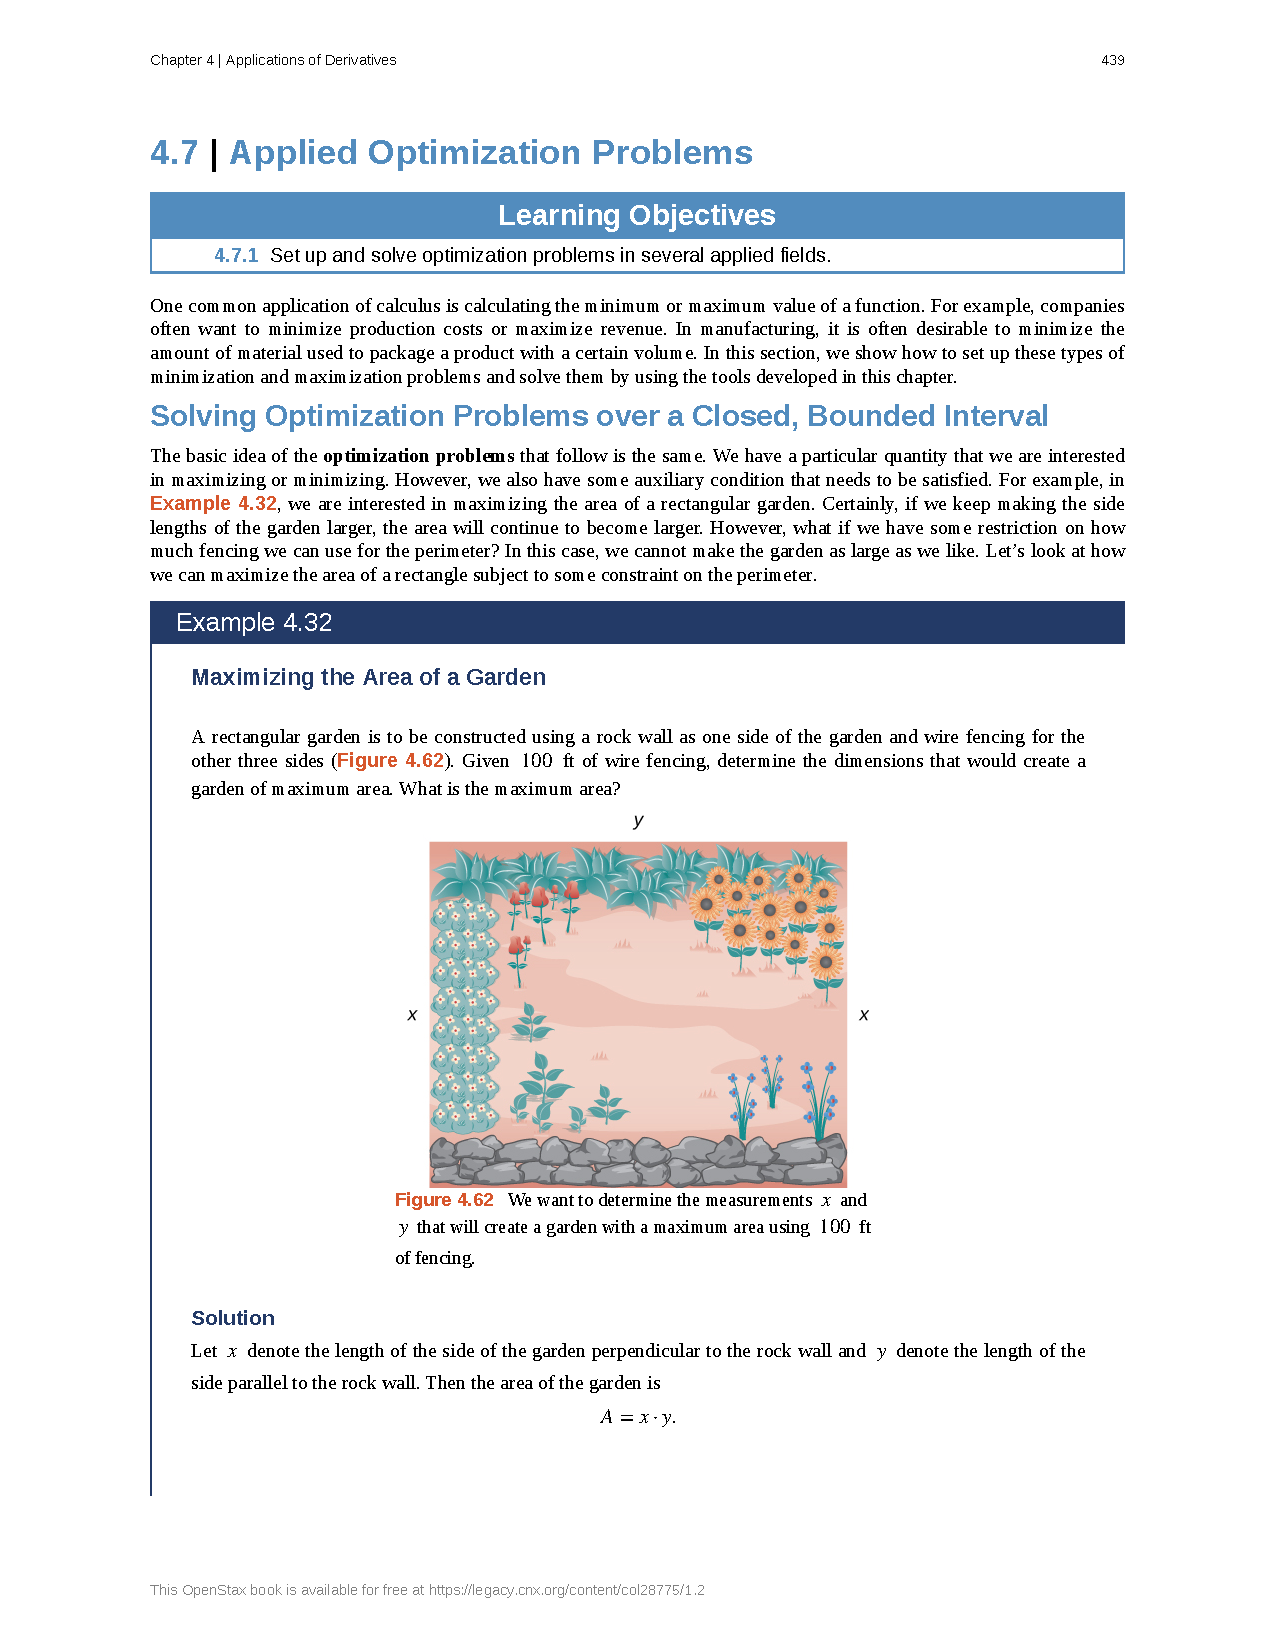
\includepdf[page={1-2}]{extras30/appliedoptimizationexample.pdf}

\end{document}